\documentclass{standalone}
\usepackage{tikz}
\usetikzlibrary{patterns, positioning}


\begin{document}
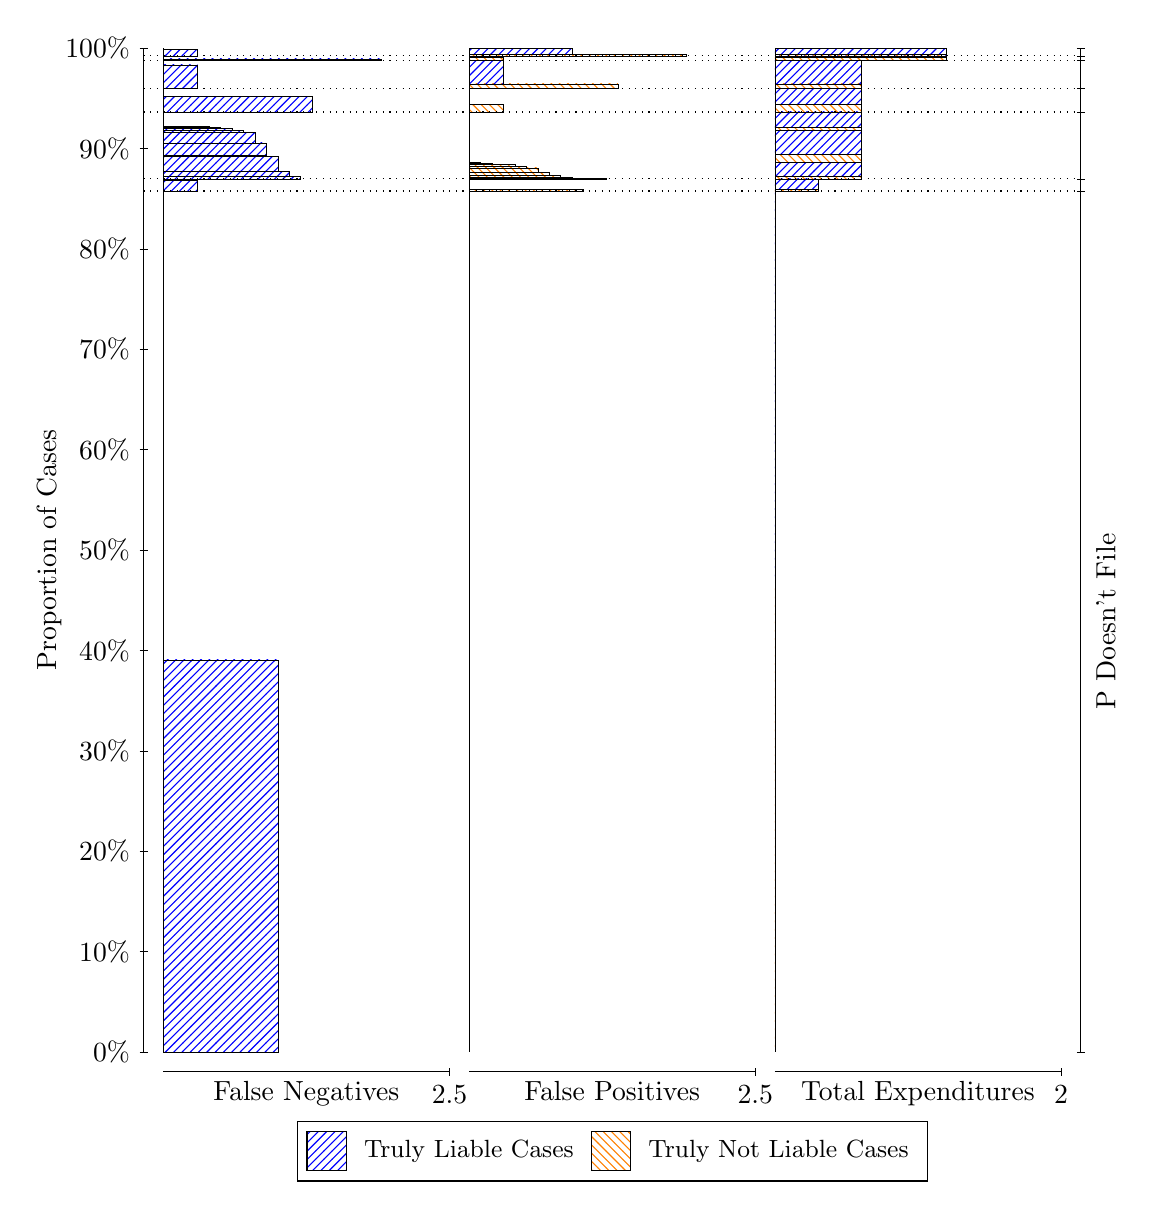
\begin{tikzpicture}
\draw[black, very thin] (1.5,1.75) -- (1.5,14.5);
\node[rotate=90, text=black, anchor=center] at (0.3, 8.125) {Proportion of Cases};
\draw[black, very thin] (1.45,1.75) -- (1.55,1.75);
\node[text=black, anchor=east] at (1.45, 1.75) {0\%};
\draw[black, very thin] (1.45,3.025) -- (1.55,3.025);
\node[text=black, anchor=east] at (1.45, 3.025) {10\%};
\draw[black, very thin] (1.45,4.3) -- (1.55,4.3);
\node[text=black, anchor=east] at (1.45, 4.3) {20\%};
\draw[black, very thin] (1.45,5.575) -- (1.55,5.575);
\node[text=black, anchor=east] at (1.45, 5.575) {30\%};
\draw[black, very thin] (1.45,6.85) -- (1.55,6.85);
\node[text=black, anchor=east] at (1.45, 6.85) {40\%};
\draw[black, very thin] (1.45,8.125) -- (1.55,8.125);
\node[text=black, anchor=east] at (1.45, 8.125) {50\%};
\draw[black, very thin] (1.45,9.4) -- (1.55,9.4);
\node[text=black, anchor=east] at (1.45, 9.4) {60\%};
\draw[black, very thin] (1.45,10.675) -- (1.55,10.675);
\node[text=black, anchor=east] at (1.45, 10.675) {70\%};
\draw[black, very thin] (1.45,11.95) -- (1.55,11.95);
\node[text=black, anchor=east] at (1.45, 11.95) {80\%};
\draw[black, very thin] (1.45,13.225) -- (1.55,13.225);
\node[text=black, anchor=east] at (1.45, 13.225) {90\%};
\draw[black, very thin] (1.45,14.5) -- (1.55,14.5);
\node[text=black, anchor=east] at (1.45, 14.5) {100\%};

\draw[black, very thin] (13.4,1.75) -- (13.4,14.5);
\draw[black, very thin] (13.35,1.75) -- (13.45,1.75);
\node[anchor=west] at (13.35, 1.75) {};
\draw[black, very thin] (13.35,12.684) -- (13.45,12.684);
\node[anchor=west] at (13.35, 12.684) {};
\draw[black, very thin] (13.35,12.838) -- (13.45,12.838);
\node[anchor=west] at (13.35, 12.838) {};
\draw[black, very thin] (13.35,13.688) -- (13.45,13.688);
\node[anchor=west] at (13.35, 13.688) {};
\draw[black, very thin] (13.35,13.988) -- (13.45,13.988);
\node[anchor=west] at (13.35, 13.988) {};
\draw[black, very thin] (13.35,14.342) -- (13.45,14.342);
\node[anchor=west] at (13.35, 14.342) {};
\draw[black, very thin] (13.35,14.401) -- (13.45,14.401);
\node[anchor=west] at (13.35, 14.401) {};
\draw[black, very thin] (13.35,14.5) -- (13.45,14.5);
\node[anchor=west] at (13.35, 14.5) {};

\draw[black, very thin, pattern color=blue, pattern=north east lines] (1.75,1.75) rectangle (3.2033,6.7281);
\draw[black, very thin, pattern color=orange, pattern=north west lines] (1.75,6.7281) rectangle (1.75,12.684);
\draw[black, very thin, pattern color=blue, pattern=north east lines] (1.75,12.684) rectangle (2.186,12.82);
\draw[black, very thin, pattern color=orange, pattern=north west lines] (1.75,12.82) rectangle (1.75,12.838);
\draw[black, very thin, pattern color=blue, pattern=north east lines] (1.75,12.838) rectangle (3.494,12.867);
\draw[black, very thin, pattern color=blue, pattern=north east lines] (1.75,12.867) rectangle (3.3487,12.93);
\draw[black, very thin, pattern color=blue, pattern=north east lines] (1.75,12.93) rectangle (3.2033,13.127);
\draw[black, very thin, pattern color=blue, pattern=north east lines] (1.75,13.127) rectangle (3.058,13.138);
\draw[black, very thin, pattern color=blue, pattern=north east lines] (1.75,13.138) rectangle (3.058,13.294);
\draw[black, very thin, pattern color=blue, pattern=north east lines] (1.75,13.294) rectangle (2.9127,13.43);
\draw[black, very thin, pattern color=blue, pattern=north east lines] (1.75,13.43) rectangle (2.7673,13.458);
\draw[black, very thin, pattern color=blue, pattern=north east lines] (1.75,13.458) rectangle (2.622,13.481);
\draw[black, very thin, pattern color=blue, pattern=north east lines] (1.75,13.481) rectangle (2.4767,13.492);
\draw[black, very thin, pattern color=blue, pattern=north east lines] (1.75,13.492) rectangle (2.3313,13.503);
\draw[black, very thin, pattern color=orange, pattern=north west lines] (1.75,13.503) rectangle (1.75,13.688);
\draw[black, very thin, pattern color=blue, pattern=north east lines] (1.75,13.688) rectangle (3.6393,13.887);
\draw[black, very thin, pattern color=orange, pattern=north west lines] (1.75,13.887) rectangle (1.75,13.988);
\draw[black, very thin, pattern color=blue, pattern=north east lines] (1.75,13.988) rectangle (2.186,14.286);
\draw[black, very thin, pattern color=orange, pattern=north west lines] (1.75,14.286) rectangle (1.75,14.342);
\draw[black, very thin, pattern color=blue, pattern=north east lines] (1.75,14.342) rectangle (4.5113,14.362);
\draw[black, very thin, pattern color=orange, pattern=north west lines] (1.75,14.362) rectangle (1.75,14.401);
\draw[black, very thin, pattern color=blue, pattern=north east lines] (1.75,14.401) rectangle (2.186,14.479);
\draw[black, very thin, pattern color=orange, pattern=north west lines] (1.75,14.479) rectangle (1.75,14.5);
\draw[black, very thin, pattern color=orange, pattern=north west lines] (5.6333,1.75) rectangle (5.6333,7.7061);
\draw[black, very thin, pattern color=blue, pattern=north east lines] (5.6333,7.7061) rectangle (5.6333,12.684);
\draw[black, very thin, pattern color=orange, pattern=north west lines] (5.6333,12.684) rectangle (7.0867,12.702);
\draw[black, very thin, pattern color=blue, pattern=north east lines] (5.6333,12.702) rectangle (5.6333,12.838);
\draw[black, very thin, pattern color=orange, pattern=north west lines] (5.6333,12.838) rectangle (7.3773,12.841);
\draw[black, very thin, pattern color=orange, pattern=north west lines] (5.6333,12.841) rectangle (7.232,12.843);
\draw[black, very thin, pattern color=orange, pattern=north west lines] (5.6333,12.843) rectangle (7.0867,12.848);
\draw[black, very thin, pattern color=orange, pattern=north west lines] (5.6333,12.848) rectangle (6.9413,12.855);
\draw[black, very thin, pattern color=orange, pattern=north west lines] (5.6333,12.855) rectangle (6.796,12.885);
\draw[black, very thin, pattern color=orange, pattern=north west lines] (5.6333,12.885) rectangle (6.6507,12.921);
\draw[black, very thin, pattern color=orange, pattern=north west lines] (5.6333,12.921) rectangle (6.5053,12.978);
\draw[black, very thin, pattern color=orange, pattern=north west lines] (5.6333,12.978) rectangle (6.36,13.001);
\draw[black, very thin, pattern color=orange, pattern=north west lines] (5.6333,13.001) rectangle (6.2147,13.023);
\draw[black, very thin, pattern color=blue, pattern=north east lines] (5.6333,13.023) rectangle (5.924,13.034);
\draw[black, very thin, pattern color=blue, pattern=north east lines] (5.6333,13.034) rectangle (5.7787,13.044);
\draw[black, very thin, pattern color=blue, pattern=north east lines] (5.6333,13.044) rectangle (5.6333,13.688);
\draw[black, very thin, pattern color=orange, pattern=north west lines] (5.6333,13.688) rectangle (6.0693,13.788);
\draw[black, very thin, pattern color=blue, pattern=north east lines] (5.6333,13.788) rectangle (5.6333,13.988);
\draw[black, very thin, pattern color=orange, pattern=north west lines] (5.6333,13.988) rectangle (7.5227,14.044);
\draw[black, very thin, pattern color=blue, pattern=north east lines] (5.6333,14.044) rectangle (6.0693,14.342);
\draw[black, very thin, pattern color=orange, pattern=north west lines] (5.6333,14.342) rectangle (6.0693,14.38);
\draw[black, very thin, pattern color=blue, pattern=north east lines] (5.6333,14.38) rectangle (5.6333,14.401);
\draw[black, very thin, pattern color=orange, pattern=north west lines] (5.6333,14.401) rectangle (8.3947,14.421);
\draw[black, very thin, pattern color=blue, pattern=north east lines] (5.6333,14.421) rectangle (6.9413,14.5);
\draw[black, very thin, pattern color=orange, pattern=north west lines] (9.5167,1.75) rectangle (9.5167,7.7061);
\draw[black, very thin, pattern color=blue, pattern=north east lines] (9.5167,7.7061) rectangle (9.5167,12.684);
\draw[black, very thin, pattern color=orange, pattern=north west lines] (9.5167,12.684) rectangle (10.062,12.702);
\draw[black, very thin, pattern color=blue, pattern=north east lines] (9.5167,12.702) rectangle (10.062,12.838);
\draw[black, very thin, pattern color=orange, pattern=north west lines] (9.5167,12.838) rectangle (10.607,12.876);
\draw[black, very thin, pattern color=blue, pattern=north east lines] (9.5167,12.876) rectangle (10.607,13.047);
\draw[black, very thin, pattern color=orange, pattern=north west lines] (9.5167,13.047) rectangle (10.607,13.151);
\draw[black, very thin, pattern color=blue, pattern=north east lines] (9.5167,13.151) rectangle (10.607,13.451);
\draw[black, very thin, pattern color=orange, pattern=north west lines] (9.5167,13.451) rectangle (10.607,13.494);
\draw[black, very thin, pattern color=blue, pattern=north east lines] (9.5167,13.494) rectangle (10.607,13.688);
\draw[black, very thin, pattern color=orange, pattern=north west lines] (9.5167,13.688) rectangle (10.607,13.788);
\draw[black, very thin, pattern color=blue, pattern=north east lines] (9.5167,13.788) rectangle (10.607,13.988);
\draw[black, very thin, pattern color=orange, pattern=north west lines] (9.5167,13.988) rectangle (10.607,14.044);
\draw[black, very thin, pattern color=blue, pattern=north east lines] (9.5167,14.044) rectangle (10.607,14.342);
\draw[black, very thin, pattern color=orange, pattern=north west lines] (9.5167,14.342) rectangle (11.697,14.38);
\draw[black, very thin, pattern color=blue, pattern=north east lines] (9.5167,14.38) rectangle (11.697,14.401);
\draw[black, very thin, pattern color=orange, pattern=north west lines] (9.5167,14.401) rectangle (11.697,14.421);
\draw[black, very thin, pattern color=blue, pattern=north east lines] (9.5167,14.421) rectangle (11.697,14.5);
\draw[black, dotted] (1.5,12.684) -- (13.4,12.684);
\draw[black, dotted] (1.5,12.838) -- (13.4,12.838);
\draw[black, dotted] (1.5,13.688) -- (13.4,13.688);
\draw[black, dotted] (1.5,13.988) -- (13.4,13.988);
\draw[black, dotted] (1.5,14.342) -- (13.4,14.342);
\draw[black, dotted] (1.5,14.401) -- (13.4,14.401);
\draw[black, very thin] (1.75,1.5) -- (5.3833,1.5);
\node[text=black, anchor=north] at (3.5667, 1.5) {False Negatives};
\draw[black, very thin] (5.3833,1.45) -- (5.3833,1.55);
\node[text=black, anchor=north] at (5.3833, 1.45) {2.5};

\draw[black, very thin] (5.6333,1.5) -- (9.2667,1.5);
\node[text=black, anchor=north] at (7.45, 1.5) {False Positives};
\draw[black, very thin] (9.2667,1.45) -- (9.2667,1.55);
\node[text=black, anchor=north] at (9.2667, 1.45) {2.5};

\draw[black, very thin] (9.5167,1.5) -- (13.15,1.5);
\node[text=black, anchor=north] at (11.333, 1.5) {Total Expenditures};
\draw[black, very thin] (13.15,1.45) -- (13.15,1.55);
\node[text=black, anchor=north] at (13.15, 1.45) {2};

\node[text=black, centered, rotate=90] at (13.72, 7.2171) {P Doesn't File};







\draw (7.449999999999999,1.5) node[draw=none] (baseCoordinate) {};
\begin{scope}[align=center]
        \matrix[scale=0.5, draw=black, below=0.5cm of baseCoordinate, nodes={draw}, column sep=0.1cm]{
            \node[rectangle, draw, minimum width=0.5cm, minimum height=0.5cm, pattern color=blue, pattern=north east lines] {}; &
            \node[draw=none, font=\small, text=black] (B) {Truly Liable Cases}; &
            \node[rectangle, draw, minimum width=0.5cm, minimum height=0.5cm, pattern color=orange, pattern=north west lines] {}; &
            \node[draw=none, font=\small, text=black] (B) {Truly Not Liable Cases}; \\
            };
\end{scope}

\end{tikzpicture}
\end{document}